\documentclass[conference]{IEEEtran}
%\usepackage[latin1]{inputenc}
\usepackage{amsmath}
\usepackage{amsfonts}
\usepackage{amssymb}
\usepackage{graphicx}
\usepackage{epstopdf}
\usepackage{AMMALanguages}
\usepackage[table]{xcolor}
\usepackage{tabularx}
\usepackage{booktabs}
\usepackage{cleveref}
\usepackage{url}

\usepackage[normalem]{ulem} % for \sout
\usepackage{xcolor}
\definecolor{colgray}{gray}{0.75}

% Put edit comments in a really ugly standout display
\usepackage{ifthen}
\usepackage{amssymb}
\newboolean{showcomments}
\setboolean{showcomments}{true} % toggle to show or hide comments
\ifthenelse{\boolean{showcomments}}
  {\newcommand{\nb}[2]{
    \fcolorbox{gray}{yellow}{\bfseries\sffamily\scriptsize#1}
    {$\blacktriangleright$#2$\blacktriangleleft$}
   }
   \newcommand{\version}{\emph{\scriptsize$-$working$-$}}
  }
  {\newcommand{\nb}[2]{}
   \newcommand{\version}{}
  }

\newcommand\rs[1]{\nb{levi}{\textsl{#1}}}
\newcommand\mf[1]{\nb{manuel}{\textsl{#1}}}
\newcommand\mc[1]{\nb{bentley}{\textsl{#1}}} 




\newcommand{\chunk}[2]{%
	\fcolorbox{black}{yellow}{\bfseries\sffamily\scriptsize#1}%
   {$\blacktriangleright$#2$\blacktriangleleft$}%
}

\newcommand{\bentley}[1]{\chunk{Bentley}{\textbf{\textcolor{green}{\textsl{#1}}}}}
\newcommand{\levi}[1]{\chunk{Levi}{\textbf{\textcolor{red}{\textsl{#1}}}}}
\newcommand{\manuel}[1]{\chunk{Manuel}{\textbf{\textcolor{blue}{\textsl{#1}}}}}
\newcommand{\javi}[1]{\chunk{Javi}{\textbf{\textcolor{brown}{\textsl{#1}}}}}

\begin{document}
\title{SyVOLT - A Model Transformation Verifier}
%\title{Full Verification of Model Transformation Contracts for Declarative ATL}
\author{Levi L\'{u}cio, Bentley James Oakes, Claudio Gomes, Hans Vangheluwe}

\author{\IEEEauthorblockN{Levi L\'{u}cio\IEEEauthorrefmark{1},
			Bentley James Oakes\IEEEauthorrefmark{1}, and
			Claudio Gomes\IEEEauthorrefmark{2}}
		\IEEEauthorblockA{\IEEEauthorrefmark{1}School of Computer Science,
			McGill University,
			Canada\\ levi@cs.mcgill.ca, bentley.oakes@mail.mcgill.ca}
		\IEEEauthorblockA{\IEEEauthorrefmark{2}MSDL Lab,
			U of Antwerp,
			Antwerp\\ \{claudio\}@internet}
	}

\date{\today}


\maketitle

%\tableofcontents



\begin{abstract}


We introduce SyVOLT, a plugin for the Eclipse development environment for the verification of structural contracts on model transformations. The plugin allows the user to build transformations in our transformation language DSLTrans using a visual editor. The pre-/post- condition contracts to be proved on the transformation can also be built in a similar interface.

Our contract proving process is exhaustive, meaning that if a contract is said to hold, then the contract will hold for all input models of a transformation. If the contract will not hold, then the input model counter-examples where the contract fails will be presented.

Demo: \url{https://www.youtube.com/watch?v=8PrR5RhPptY}



\end{abstract}


\section{Introduction}
\label{sec:intro}
%\subsection{Model Transformations}

% MDD and MTs. Not very important but I do not know how far back should we start.
Model-Driven Development (MDD) is a software engineering approach that uses
models - typically represented as graphs - as first class citizens to create and evolve software systems
\cite{Hailpern:2006vd}.
Model Transformations, prescribed by Model Transformation Languages (MTLs) are the preferred approach to manipulate those models \cite{Software2003}.
MTLs typically describe a set of rules that guide the transformation of models.
Their productivity comes from the fact that those rules can be described
elegantly without the accidental complexity of graph manipulation.\markus{This
last sentence sounds weak and unclear. What is the point?}

% Model translations vs Rewritting Transformations.
Here\markus{where is here? In this paper?}, a model transformation is defined as
a translation, as opposed to a graph rewriting process.
In graph rewriting, a graph representing a model or a set of models\markus{Why
is the ``set'' important here?} gets rewritten continuously according to a set
of rules, until some termination criteria is met.
In a model translation, there is a source model and a target model and the
target model is the result of applying the translation to the source model.
Operationally speaking, each of these approaches can mimic the other: graph
rewriting can be used to perform model translations (e.g. \cite{Grunske2005})
and model translations, \emph{when applied repetitively}, can perform graph
rewriting.\markus{I presume you explain this because it will become important
later. If so, please give the reader a hint. In not, remove it.}


\subsection{Model Transformation Verification}

% What is transformation verification?
Notice that the previous property is in the form of an implication, which must
be true independently of the concrete input model given to the transformation.
This means that to prove the property, it is not enough to prove that it holds
for a single input model with a father, a mother, a son and a daughter. That
would be just \emph{testing} the transformation.
Rather, we must \emph{prove} that it holds for the infinitely many\markus{I
know what you want to say. But it's not really about the *many* right? It is
about all possible input models.} possible input models.

% Motivation for automatic verification
For small transformations it is easy to prove that they satisfy certain
properties. However, model transformations have been successfully applied in
industry (e.g., \cite{daghsen:hal-00660252,Giese2010}) and these transformations
-- and the models involved, as evidenced in \cite{Selim2012} and in our own case
study Section~\ref{sec:mbeddr_case_study} -- can be quite large
\footnote{Transformations with circa 50 rules and metamodels with more than 1500
classes}.
For these transformations, automatically proving their correctness is of
utmost importance.\markus{Why?}

%bridge to the next section.
By correct transformations, we mean that they are automatically proven to satisfy the properties described by the domain expert. We abstain from prescribing which properties are of interest. Instead, we focus on the verification/proving process itself.

\subsection{SyVOLT Contract Verification Tool}

Our approach to model transformation verification is based on a contract-based technique. Our tool is SyVOLT (Symbolic Verifier of mOdeL Transformations) which represents all possible transformation executions using a symbolic execution approach. ADD ADD

\subsection{Paper Structure}

This paper will therefore discuss our tool for verifying structural contracts on sizable transformations. First, we begin by describing DSLTrans and an introductory example in Section...



\section{Highlights}
\label{sec:highlights}
%SyVOLT (Symbolic Verifier of mOdeL Transformations) is a user-friendly
Eclipse plugin to verify pre-/post- condition contracts on model transformations
specified in the DSLTrans transformation language. The tool has a number of
unique features, outlined below.

\subsection{Graphical Modelling of Model Transformation Contracts}

SyVOLT proves pre-/post-condition contracts hold for a model transformation.
Such contracts establish relations between patterns occurring in input and output
models of a model transformation. If a contract holds, then a formal guarantee
exists that whenever an input model contains the pattern specified in the
pre-condition of the contract, the output model contains the pattern specified
in the post-condition part of the contract and any traceability relations
between the two. Due to the graph-like structure of the pre and post conditions
of contracts, the visual representation of the contract in SyVolt editor allows
the user to quickly build and intuitively understand their meaning.
If a textual (logical or mathematical) editor where to be used, the user would
need an extra system of identifiers to correctly prescribe the associations between pre and post-condition elements whereas in the visual representation, the user graphically builds the associations between those elements.
\levi{Claudio, I don't understand this sentence}
\cgg{Please tell me now if you can understand it.}

The visual representation of a contract has all the necessary information to derive the correct 
logical expression to be used by the internal SyVolt prover.

\subsection{Push-Button Proofs}
\label{sec:push_button_proofs}
SyVOLT is a verification tool that provides formal guarantees of correctness of
a model transformation. The proving process is fully automatic and
the all formal details are completely hidded from the user, who only needs to specify a
set of contracts for the transformation being verified. Once the transformation and the
contracts of interest are created, one command will start the property proving
process. This process will automatically create all required artifacts (as
detailed in the following section), run the process, and then provide the
results to the user within the Eclipse environment, as seen in
Figure~\ref{fig:output}. This allows the user to continually stay within the
Eclipse environment, which is where he develops the contracts and the model
transformations.

\subsection{Based on Symbolic Execution}

Our technique shares its principles with symbolic execution, a
classically used method to verify code. The underlying idea entails building a
finite representation of the (infinite) set of model transformation
computations, such that properties of interest can be proved on such finite
representation and extrapolated to the infinite set of possible computations.

Our model transformation verification technique relies on typed graphs as the
means to internally represent both symbolic executions and contracts. SyVOLT
then reasons over these graphs to build a proof that contracts hold or do not
hold. Note that by using a typed graph representation, our technique can prove
contracts that include constraints on the attributes of the input and output
models.

\levi{keep the text from here on?} An example of this would be in the
Families-To-Persons transformation from the ATL zoo [CITE]. In this transformation, the name for a person in the
output graph is a concatenation of two strings \cgg{instead of ''strings``,
should be ''attributes``} from elements in the input graph. Our contract prover
can prove that this concatenation will be valid in all cases.

\begin{figure}
\centering
\includegraphics[width=0.45\textwidth]{figures/output}
\caption{The results of the contract prover}
\label{fig:output}
\end{figure}

\subsection{Input Independence and Exhaustiveness} 

Our technique is exhaustive, in the sense that whenever a contract holds, it
will hold for all possible input models to a transformation. This is possible
because SyVOLT operates on specifications of outplace model transformations
where unbounded loops and model element deletions are not allowed. SyVOLT thus proves
contracts in an input-independent manner, relying only on the specification of the
transformation. The soundness and completeness of our technique is described
in~\cite{Lucio2014}.

\subsection{Proving Contracts about ATL Model Transformations}
The Atlas Transformation Language (ATL) is commonly-used in both industry and
academia applications. In order to extend our approach into these domains, we
have developed a higher-order transformation that is able to automatically
transform declarative ATL transformations into our transformation language
DSLTrans~\cite{Oakes}. This allows the user to also prove contracts on
ATL transformations.

\subsection{Scalability and Speed}

We have some evidence that SyVOLT scales to transformations of practical
interest. This has been empirically shown by applying it to DSLTrans
transformations up to over 60 rules, and ATL transformations up to 13
rules~\cite{Oakes}. From our own experience with DSLTrans, the size of a
DSLTrans transformations varies widely, with the average size ranging from 10 up
to 50 rules. The average size of an ATL transformation is around 20 rules. [cite
Manuel's paper, should we keep this?].
Even though our technique is exhaustive, our approach takes relatively short
amounts of time to prove contracts. For example, our experiments with industrial
transformations~\cite{Oakes} show that contracts can be verified within a few
minutes. In Gehan Selim's PhD thesis~\cite{Selim2015}
further evidence of SyVOLT's speed is given when verifying a relatively large
model transformation for giving semantics to the UML-RT language in terms of
the Kiltera process language~\cite{PosseDingel2014}. SyVOLT's symbolic execution
engine is fully homegrown~\cite{LucioVang} and does not depend on third-party
solvers. Although this has implied a large effort to build the codebase, it has
also allowed us to have the required control over the code to iteratively
optimize the engine for both space and time economy. \cite{Selim2014}
demonstrates that our prover is substantially faster than similar approaches based on SAT solvers.


\subsection{Production of Counter-Examples}

When a contract is proved to be violated by a given model transformation, it is
useful to also provide an input model - called a \emph{counter-example} - so
that the user can execute the model transformation with that input and verify
that indeed it violates the contract.

An advantage of out technique is that the counter-example produced by SyVolt
describes a family of input models that violate the contract. This means that
any input model that belongs to the family of the counter-example - i.e., fits
the description given by the contract proving process - causes the model
transformation to violate the contract. \cgg{Levi, did you also show that any
model that does not belong to the family does not cause the model transformation
to violate the contract?} Thus, the user can easily determine the error in the
transformation and correct it. We suggest that this supports a transformation
development method analogous to 'test-driven development'. In this method,
development would be routinely punctuated by contract proof in order to catch
errors early and store test cases - the counter examples produced - to be used
in the future.


\subsection{Integration with Eclipse}

Eclipse is a popular development environment and model transformation
tools such as ATL [CITE], DSLTrans [CITE] and EGL [CITE] are integrated with the
Eclipse Modeling Framework (EMF) [CITE].

To take advantage of this ecosystem, SyVolt integrates with EMF.
In the EMF, models can be represented in a multitude of syntaxes, from graphical
to textual, and this makes the interaction with SyVolt easier since the modeler
can use the model editor that is most convenient. Internally, SyVolt uses 
the Himesis format [CITE] to represent models.

%\subsection{Model Driven Developed GUI\levi{this text is subsumed by section
%III a)}}
%\label{sec:mdd_gui}

%To take advantage of the productivity promised by MDD, we used a language
% called Eugenia[CITE] to develop the SyVolt contract editor shown in
%Figure~\ref{fig:eclipse_frontend}.
%With this approach, the SyVolt editor was developed in about 4 man-hours.

\begin{figure}
\centering
\includegraphics[width=0.45\textwidth]{figures/eclipse_frontend}
\caption{The transformation editor within Eclipse}
\label{fig:eclipse_frontend}
\end{figure}




 

\section{Architecture}
\label{sec:arch}
%\begin{figure*}
\centering
\includegraphics[width=0.8\textwidth]{figures/syvolt_arch}
\caption{The architecture of the SyVOLT tool}
\label{fig:arch}
\end{figure*}

The guiding principle of the Modelling, Design, and Simulation Lab is that all
tools and processes should be explicitly modelled at an appropriate abstraction level.
This practice goes in the direction of ensuring that essential
complexity is the main object of software development and that accidental
complexity is mitigated as much as possible.

SyVOLT's codebase has been developed by applying these principles. We have used
available model-driven development technology as much as possible, both to
develop and as a part of SyVOLT itself. In particular, we have made it such
that the representations of the DSLTrans transformations and the SyVOLT
contracts manipulated by the proof engine are models. The representations of symbolic
executions produced for a given DSLTrans model transformation, also called
\emph{path conditions}, are equally models. Moreover, given the operations
required by the algorithm for building a contract proof (described in~\cite{Lucio2014}) can be implemented as model
manipulations, we have operationally encoded them as model transformations.
In~\cite{LucioVang} how we explain how we use \emph{model transformations to
verify model transformations} in our contract prover.\\

The following model-driven development tools have been used either as part of
SyVOLT's codebase, or for SyVOLT's development:
\begin{itemize}

  \item \textbf{AToM$^3$}~\cite{}: AToM$^3$ is a meta-editor for model-driven
  development. It has been developed at the MSDL and is used for constructing,
  models, metamodels and model transformation rules, and for automatically
  synthesising modeling environments.
  AToM$^3$ has been extensively used to give support to the construction and
  visualisation of models and model transformation rules required by the proof
  engine during the initial stages of the construction of SyVOLT. 
  Many of these artifacts were explicitely built during the construction
  of SyVOLT in order to develop and test the proof algorithm in a controlled
  environment. In the finished SyVOLT all these artifacts are automatically
  generated from their graphical representations in the Eclipse front-end.\\

  \item \textbf{Himesis}~\cite{Provost2006}: Himesis is a typed graph representation
  format, built upon the open-source igraph~\cite{} library. 
Himesis is used for several reasons: independence, efficiency and tool support.
Independence is ensured because Himesis is very expressive and also very simple,
which means it will not change for the foreseeable future.
In \cite{Syriani2010b}, it is reported empirically that Himesis is a good format
to perform the typical graph manipulation operations and it is seamlessly
supported by T-Core.  
  Himesis is used pervasively within SyVOLT to represent models of 
  DSLTrans rules and of SyVOLT contracts, as well as all the model
  transformation rules required by the proof algorithm.\\
  
  \item \textbf{T-Core}~\cite{Syriani2010a}: T-Core is a collection of model transformation
  primitives developed at the MSDL, allowing fine-grained manipulation of
  models. It was initially built as a means to rapidly build
  high-level model transformation languages. T-Core has been used to
  successfully deconstruct and reconstruct several mainstream model transformation
  languages~\cite{}. The main operations of T-Core are model \emph{matching},
  model \emph{rewriting} and \emph{iterating} through a set of match sites in a model.
  The level of control in model manipulation, together with T-Core's speed and
  scalability when treating large models, suited well our needs when
  implementing the property proof algorithm described in~\cite{Lucio2014}. Note that because
  T-Core is also an explicitly modeled model transformation language, a T-Core
  model transformation rule is also a (Himesis) model.\\

  \item \textbf{EMF} (Eclipse Modelling Framework)~\cite{}: SyVOLT makes use of
  EMF's E-Core format for the XMI~\footnote{\url{http://www.omg.org/spec/XMI/}} representation of DSLTrans transformations
  and SyVOLT's contracts within the Eclipse editors. Note that EMF is only used
  in the Eclipse front-end, and that Ecore models are converted into
  the Himesis format for the contract prover engine to compute the
  proofs.\\
  \item \textbf{EGL} (Epsilon Generation Language)~\cite{}: Converting Ecore
  models into Himesis models is achieved using EGL, a language from the Epsilon
  family. Besides easy integration with Eclipse and native support of the expressive
Epsilon Object Language (EOL~\cite{Kolovos}), EGL also provides tasks for the
Ant~\footnote{\url{http://ant.apache.org}} build tool, which was used to
orchestrate the multiple tools in the proving process (see
Section~\ref{sec:push_button_proofs}).\\
\end{itemize}

% Elements of the architecture that could not be built using model driven tools
% (for lack of technological availability) have been developed using model-driven
% principles.

Figure~\ref{fig:arch} shows the architecture of the SyVOLT tool. Two essential
blocks are depicted: the graphical Eclipse front-end and the proof engine
back-end. While the front-end is responsible for the interaction with SyVOLT's
user, the back-end implements the algorithm for running the proofs of the contracts. Note
that two kinds of communication occur between SyVOLT's front-end and back-end:
in the left-to-right direction, a number of artifacts (models and model
transformations) are syntesized from the graphical representations of the
DSLTrans transformations and of the SyVOLT contracts, and passed to the
back-end.
In the reverse direction, the proof result and counter-examples, if any, are
passed from the proof engine back-end to the Eclipse front-end.

Note that in Figure~\ref{fig:arch}, each component is annotated by a number
identifier. Following this numbering sequence, we will briefly visit each
component to describe its function and the technologies employed in its development.

SyVOLT's architectural components described in Figure~\ref{fig:arch} are
orchestrated by an ANT script from within Eclipse. This script makes sure all components execute in the
right order, provides the glue between them and allows contract proof to run at
the push of a button and without any intervention from the part of the user.


% In particular, each artifact and transformation in the contract prover is
% explicitly modelled. EXPAND

% Present:
% \begin{itemize}
%   \item Technology used: introduce orthogonal technologies used in all
%   static components
%   \item Static components
%   \item Flow
% \end{itemize}
% 
% The contract prover makes heavy use of T-Core [CITE], which is a framework of
% transformation primitives. For example, the T-Core Matcher and Rewriter is
% scheduled by Python in order to perform rewriting on a graph in an efficient
% manner.


\subsection{SyVOLT Contract Editor (1)}\levi{too heavy on how it was
developed and tool little on how it is used}

The SyVolt contract editor is realized by a set of Eclipse plugins.
The runtime architecture of this editor is the typical architecture of a
Graphical Modeling Framework (GMF)
\footnote{\url{http://www.eclipse.org/modeling/gmp/}} editor.
What is important is how this editor was developed.

As mentioned in Section~\ref{sec:mdd_gui}, we used Eugenia[CITE] to quickly
develop the SyVolt contract editor shown in Figure~\ref{fig:eclipse_frontend}.

Eugenia consists of a set of annotations that are attached to the metamodel of
SyVOLT contracts. An annotation can, for instance, specify that an atomic
contract will be drawn as a rounded rectangle, with a specific color and a label
that is equal to the name attribute of the contract.
The annotations are not very expressive but they contain the essential
information to generate a set of GMF models that, ultimately, describe a basic
usable graphical editor.

Each generated GMF model is concerned with one aspect of the editor and can be
further customized to our needs. GMF models are much more expressive than the
Eugenia annotations.
For instance, the generated GMF tooling model prescribes the kind of tools that
will be available in the toolbox (shown in the right of
Figure~\ref{fig:eclipse_frontend}), their icons, labels, etc\ldots

From the set of GMF models, a set of eclipse plugins are synthesized.
These make up SyVolt graphical editor\footnote{A fixed structure textual editor
is also provided but this editor lacks several usability improvements and,
hence, is not appropriate to model SyVolt contracts.}.

The original DSLTrans transformation is manipulated using the DSLTrans editor
and is serialized in XMI format. Similarly, SyVOLT contracts are manipulated with the SyVolt graphical
editor and serialized in XMI format.


\subsection{Generating Models and Model Transformations for Proof Construction
(2)}
\label{sec:gen_models_mt}

The translation of DSLTrans transformations and SyVOLT contracts into Himesis
models and model transformation rules was achieved using the Epsilon Generation
Language (EGL~\cite{Rose2008}). More specifically, two EGL model-to-text model
transformations were used: one to generate the Himesis models
representing of a DSLTrans transformation; another one to generate the T-Core
model transformation rules necessary to prove SyVOLT contracts.

These model-to-text transformations are used to parse the Ecore models of a
DSLTrans model transformation under analysis and of the contracts to be proved.
From these Ecore models, the EGL transformations produce a number of Python
files containing classes that inherit from the Himesis library and that
represent models and T-Core transformation rules. These classes are loaded from
disk by the Python interpreter and become models and model transformations in
memory once they are instanciated by the proof engine back-end.
% Note that all these artifacts are produced as
% Python text files containing Himesis format that are needed to automatically
% perform the required proofs.
% containing models of the DSLTrans transformation being analysed
% and the T-Core model transformation rules necessary for the property proof step.

Note that, while this approach of building models and model transformations as
textual files is sufficient for our needs, it is not ideal from the model-driven
development viewpoint. Building models as textual files forces us to deal to
the accidental complexity of Python code and of the Himesis format, making the
generation of these artifacts more difficult and error prone than it needs to
be. The issues encountered here expose one of the current important fragilities
of model-driven development: the difficulty of exchanging high-level data
between different modelling frameworks~\levi{cite benoit combemale here}.


% As opposed to the XMI format which declaratively represents the graph, the
% Himesis representation of a graph is given by Python code referencing the
% Himesis library. When this code is executed it loads the Himesis graph to
% memory.

% Since Himesis is a textual format, identifiers are necessary to correctly
% describe the associations between graph nodes. The EGL transformations make sure
% these are correctly generated.


\subsection{Additional Generation of Model Transformations for Proof
Construction: The PyRamify Script (3)}

Additional model transformations, other than the ones described in
Section~\ref{sec:gen_models_mt}, need to be generated for the property proof
algorithm to execute. These are the \emph{path condition generation} T-Core
model transformations (see Figure~\ref{fig:arch}) that are needed to perform the
model manipulations for building a set of symbolic executions given a DSLTrans
model transformation. These model transformations blocks allow combining the rules of a DSLTrans model
transformation into a set of \emph{path conditions}, as per the algorithm
described in~\cite{Lucio2014}. Note that the path condition generation T-Core
transformations are fully generated from the set of rules of the DSLTrans
transformation being verified.

This additional model transformation generation step is achieved by the PyRamify
component. PyRamify is a Python script that takes as input Himesis graphs
representing the rules in the transformation. Then, through the RAMification
procedure [CITE RAM], T-Core matchers and rewriters for each rule are produced.
Very briefly, while matchers allow the contract prover to determine how
rules might execute over a path condition being built, rewriters properly
combine the right-hand side of a DSLTrans rule with that same path condition
whenever necessary.

% PyRamify is also responsible for producing additional T-Core model
% transformations used for analysing how the DSLTrans rules in a transformation
% depend on each other. Explain this further??

Currently, PyRamify is implemented as a Python script, as we were unable to
implement at the time automatic creation of higher-order artifacts (in our
case, T-Core transformations) from models in another modelling tool.
This was due to the mix of different modelling abstraction levels present in
SyVOLT and that led to a number of technical difficulties.

We have recently learned that, alternatively, \emph{path condition generation
transformations} could be built directly from the Ecore representation of
DSLTrans rules by using EGL technology -- as was done for the artifacts
described in Section~\ref{sec:gen_models_mt}. Nevertheless, a preferred solution for us would
be to use model transformation technology that that explicitely allows
building model transformations from simple models. To the best of our knowledge,
model transformation technology that allows moving between models of an order 
$n$ and an order $n+1$ is not yet available in the modelling community.

\subsection{Path Condition Generation (4)}
\label{sec:path_cond_gen}

Once the required artifacts have been produced, the prover moves onto the path
condition generation step. Each path condition will represent an (infinite) set
of concrete executions of the transformation, where each concrete execution is an
input/ouput pair. Path condition generation is operationally achieved by
executing, following the ordering of the rules in the DSLTrans
tranformation being analysed, the \emph{path condition generation transformations} generated by the
\emph{PyRamify} component. 

The path condition generation algorithm starts from the empty path condition,
representing the case where no rules in the transformation have executed. Then,
as each T-Core transformation in the \emph{path condition generation
transformations} set is executed, each rule in the DSLTrans model transformation
under analysis is combined with the path conditions generated thus far. As each
rule is considered, the set of path conditions will grow
to represent all allowed combinations rules combinations. As the execution of a
rule in a DSLTrans transformation may depend on the previous execution of other rules,
such dependencies are verified by the \emph{path condition generation
transformations} in order to exclude impossible rule combinations.

% The final set of path conditions produced by the algorithm will then abstract
% the infinite set of all concrete transformation executions. This is further
% described in~\cite{Lucio2014}, along with a formal discussion of the validity
% and completeness of this work.

Note that \emph{path condition generation} is a complex task, difficult to fully
model as a single model transformation. As such, the algorithm
has been implemented as a Python script that is responsible for scheduling all the
\emph{path condition generation transformations} in the right order. This programmatic level of granularity of
manipulation has allowed us to build many optimizations to speed up the path
condition generation process. Examples of such optimizations are the caching of
expensive match operations, or the parallelization of the path condition generation algorithm. 

\subsection{Contract Proof (5)}

Once the path conditions are generated, the proof that each
contract holds or does not hold can then be built. The \emph{contract proof}
component requires two inputs: the \emph{path conditions set} built by the path
condition generator; the \emph{property proof T-Core transformations}, generated by EGL model-to-text
transformations as described in Section~\ref{sec:gen_models_mt}.

Pre- / post- condition contracts form an implication, which needs to be
checked for each path condition provided as input to the contract proof
component. For a contract to hold on a DSLTrans model transformation, the
contract's implication should hold for every path condition generated for
that model transformation. Checking if the implication between a contract's pre-
and post- condition holds on a path condition is achieved by attempting to find for each submodel of
the path condition that is isomorphic to the pre-condition's model, a submodel
of the path condition that is isomorphic to the post-condition's model. The
computations on the existence of these sugraphs isomorphisms is done by
the \emph{T-Core property proof transformations}. Note that, in this case, the
T-Core transformations are simply a set of matchers, or queries, as no further
editing of the path conditions is necessary during this part of the proof.

As in for the path condition generation component described in
Section~\ref{sec:path_cond_gen}, the contract proof algorithm has also been
implemented as a Python script that schedules all the property proof T-Core
transformations appropriately. As before, using fine-grained programmatic
manipulations of the models and model transformations involved in the contract
proof algorithm has allowed us to implement optimization strategies. The main
of these strategies is the skipping of path conditions for which the contract
is sure to hold without further analysis, given existing cached information
about similar path conditions.



%
%\section{Mapping ATL into DSLTrans}
%\label{sec:mapping}
%\input{text/mapping}
%
%% \section{Transformation to DSLTrans}
%% \label{sec:transformation}
%% \input{text/hot}
%
%%\section{Properties and Property Prover}
%%\label{sec:prover}
%%This section will describe our proving technique, as well as present an overview of the principles and major design of the SyVOLT tool which implements this technique.

\subsection{Proving Technique}
This section will describe the operation of our contract prover such that contracts are proven on all executions of a
DSLTrans transformation.

The contract prover we describe here is the engine of
the SyVOLT tool, which can currently be used to develop and verify DSLTrans transformations within the Eclipse
environment~\cite{Lucio2015,syvoltTool,syvoltVideo}. Examples of contracts we prove are also presented, along with a brief discussion of the expressibility of the contract language.

\subsection{Contract Proving Overview}

Given a transformation written in the DSLTrans transformation language, our
contract proving technique can prove whether pre-\slash post-condition contracts will hold or
not hold on all executions of the transformation. If a contract holds, then whenever the pre-condition of the contract matches over an input model, then the post-condition of the contract will match over the corresponding output model.

  \begin{figure}[ht]
     \begin{center}
       \includegraphics[width=0.36\textwidth]{figures/FamToPersons/Pos_FourMembers.png}
       \caption{A contract to verify that two \emph{Woman} and two \emph{Man} elements are produced from the corresponding \emph{Members}}
       \label{fig:familyProp}
     \end{center}
     \vspace{-0.15in}
   \end{figure}

  For example, Figure~\ref{fig:familyProp} describes a contract to be proved over all transformation executions for the extended \FTP transformation. An informal statement for this contract is:
  \textit{`an input family with a father, mother, son and daughter should always produce
  two men and two women in the output community'}. Note that we employ backward links as part of the contract language, where as they are used to require that the output elements be
  generated from the attached input elements, similar to their use in DSLTrans rules. Our contract prover is then
  able to prove whether or not this contract will hold for all transformation executions, and produce any counter-examples if they occur. Further examples of contracts are found in Section~\ref{subsubsec:contract_examples}.


 Contracts are proved through a process that first symbolically constructs all
 possible executions of the transformation, producing a set of \emph{path conditions}. Each path condition represents the execution of a set of transformation rules, by containing the input and output elements which are produced by the execution of those transformation rules.

 For example, the path condition in Figure~\ref{fig:pc_first} represents the execution of three rules in the transformation. This representation includes the input and output elements that will be present in the input and output models if these three rules execute. The set of path conditions produced by the prover will therefore partition the set of valid executions of the transformation, where each execution is an input/output model pair. This technique was first proposed in~\cite{Lucio2010} and further detailed in~\cite{Lucio2014}.

   \begin{figure}[t]
     \begin{center}
       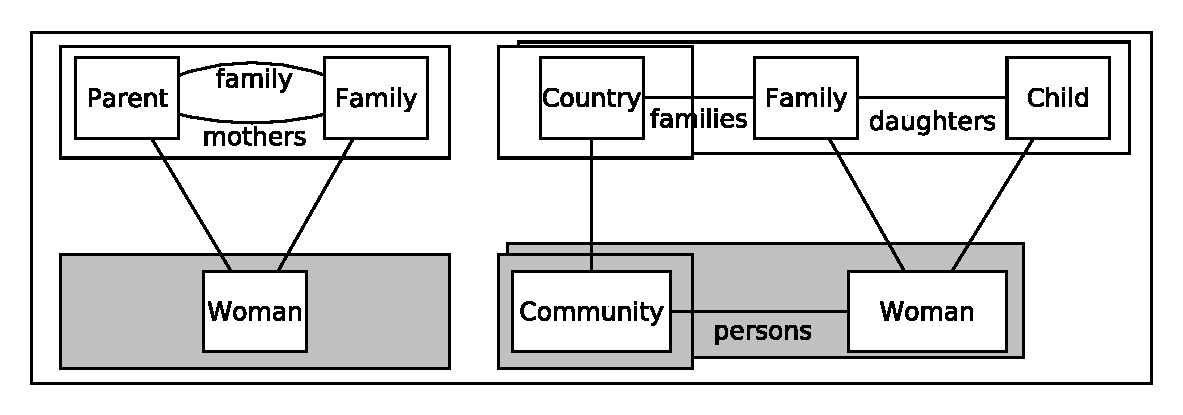
\includegraphics[width=0.45\textwidth]{figures/prover/pc}
       \caption{An example path condition representing the execution of three rules}
       \label{fig:pc_first}
     \end{center}
     \vspace{-0.20in}
   \end{figure}



 Pre-/post-condition contracts form an implication, which needs to be checked
 for each path condition that has been generated by the proving algorithm. In broad
 terms, a contract holds on a path condition if either the contract's
 pre-condition elements cannot be found in the path condition, or the contract's pre-condition
 together with its post-condition can be found in the path condition. The contract
 does not hold on the path condition if its pre-condition can be
 found in the path condition but its post-condition cannot. Finally, a contract
 holds for a transformation if it holds for all of its generated path conditions.

 Contracts are formally described in~\cite{Lucio2014}, while extensive discussion of the contract language is found in the PhD thesis of Gehan Selim~\cite{Selim2015}. Section~\ref{subsubsec:contract_examples} and Section~\ref{subsubsec:contract_results} present further contract examples, while Section~\ref{subsubsec:contract_expressiveness} briefly discusses the expressiveness of the contract language.

\subsection{Path Condition Creation}
\label{subsec:contract_prover}

As described in \cite{Lucio2015}, our contract prover constructs all artifacts used for contract proof through matching and rewriting of typed graphs. Therefore, the first step for the contract proving process is to create T-Core matcher and rewriter primitives from each of the rules
in the DSLTrans transformation~\cite{Syriani2013}. These model transformation primitives are at the core of our prover, allowing us to
reason about how rules could overlap with each other during transformation
execution, and to perform the graph rewriting necessary for our
technique.

Note that this use of reasoning about the transformation under study as explicit graphs is in opposition to other approaches in the literature, where the transformation specifications are translated into a SAT solver or theorem prover, and then the proving mechanisms for those tools are used. A further discussion of our approach versus that in the literature can be found in~\cite{Selim2015}.

In order to fully reason about all input models to a transformation, our contract prover creates a set of artifacts that represent all
possible executions of the transformation. These artifacts are created by
symbolically executing all rules in the transformation, taking into account
rule overlapping and dependencies between rules. The rule combinations that are
created are termed \textit{path conditions}.

For example, the first path
condition could represent the case where no rules in the transformation execute.
The next path condition is the case where only the first rule executes, the next
is where only the second rule executes, and a fourth path condition is where
both the two rules execute.

Note that in our path condition creation process, we
only consider one execution of each rule. That is, either a rule does not
execute (and does not appear in the path condition), or we assume that it executes some number of times (and the rule appears once). This restriction is due to our abstraction, where we symbolically represent
many executions of the same rule by the rule being present only once in each path
condition. This abstraction is necessary for analysis purposes, as the infinite number of transformation executions must be covered by a finite number of path conditions. Note that this abstraction is possible because of the
monotonicity of a DSLTrans transformation: a rule can only add elements to the
output model of a DSLTrans transformation, but never remove them.

As the transformation is made of layers, the symbolic execution process moves
through each layer and determines how rules may interact with each other. Unlike generating the powerset of all rules, these
rule interactions may in fact decrease the number of path conditions generated
by the prover as certain combinations of rules are proven infeasible.

For example, consider a rule R1 which matches on an \textit{A} element, and a
rule R2 which matches on an \textit{A} element connected to a \textit{B}
element. During an execution of the transformation, it would be impossible for R2 to execute without R1 also executing, as the match graph of R1 is a subset of the match graph of R2. Therefore, the rule R1 is `subsumed' by the rule R2. Our prover is able to detect these subsumption interactions and resolve them in a step just prior to path condition generation. This lowers the number of path conditions created by disallowing certain rule combinations, as further discussed in~\cite{Selim2014}.

As well, DSLTrans rules can also define \textit{backward links}, as described for the extended \FTP transformation in Section~\ref{sec:ATL_DSLTrans}. Recall that these backward links make dependencies on elements created by earlier rules. Specifically, these backward links require that the connected element in the
apply part of the rule was created from the connected element in the match part of the rule, by matching over traceability links created during the execution of the transformation. This functionality is therefore similar to the implicit binding step present in ATL, as discussed in Section~\ref{sec:ATL_DSLTrans} under the title \textit{Generic Semantics for Step 2}. During path condition construction, these backward link dependencies prevent some rules from executing, further decreasing the rule combinations possible.






 
%
%\section{Results and Discussion}
%\label{sec:results}
%We have some evidence that SyVOLT scales to transformations of practical
interest. This has been empirically shown by applying it to DSLTrans
transformations up to over 60 rules, and ATL transformations up to 13
rules~\cite{Oakes2016}. From our own experience with DSLTrans, the size of a
DSLTrans transformations varies widely, with the average size ranging from 10 up
to 50 rules. The average size of an ATL transformation is around 20 rules. [cite
Manuel's paper, should we keep this?].\markus{Well, if we look at the case study
in this paper (mbeddr), then we can definitely see that to really verify mbeddr,
we'll have waaay more rules.} Even though our technique is exhaustive, our
approach takes relatively short amounts of time to prove contracts. For example,
our experiments with industrial transformations~\cite{Oakes2016} show that contracts
can be verified within a few minutes. In Gehan Selim's PhD
thesis~\cite{Selim2015} further evidence of SyVOLT's performance is given when
verifying a relatively large model transformation for giving semantics to the
UML-RT language in terms of the Kiltera process language~\cite{PosseDingel2014}.
SyVOLT's symbolic execution engine is fully
homegrown~\cite{LucioVang}\markus{Does ``homegrown'' have positive connotations?
Not sure.} and does not depend on third-party solvers. Although this has implied
a large effort to build the codebase, it has also allowed us to have the
required control over the code to iteratively optimize the engine for both space
and time economy.
\cite{Selim2014} demonstrates that our prover is substantially faster than
similar approaches based on SAT solvers.
%
%
%\section{Related Work}
%\label{sec:related}
%\input{text/related}
%
%\section{Conclusion}
%\label{sec:conclusion}
%add conclusion here\ldots

Here are some ideas that should be incorpared somewhere in this journal:
\begin{itemize}
  \item Something that we should make clear in the case study section of the mbeddr: there is no way for the user of mbeddr to modify the variables that are involved in the contract. The consequence of this is that we do not need to look into the body of the executable functions created by the user of mbeddr. In particular, we do not need complicated dataflow analysis to ensure this.
  \item Can we prove that there is no other assignment being made that changes the variables involved in the hand side of the contract? 
	This is a difficult question but based on the ideas proposed by Markus, it might be possible to prove them with two contracts and an implication between them. Basically, we state the contract in other perspective: if there is any assignment changing the left hand side of the variables, then the right hand side of that very same assignment should be comprised of the correct expression. This is where the implication comes into play. We make a contract proving that any assignment must be made and the  second contract proves that that same assignment has the correct right hand side.
	\item How do we pick the most relevant contracts to be proven?
	A rule of thumb would be to look at those contracts that, if not satisfy, will result in bugs that are very hard to catch at runtime, i.e., they do not cause a crash but instead they cause mal functioning.
	This is an important rule of thumb because, as Markus said, embedded systems usually must ensure that, if they do not crash in the first seconds of operation, when a self-check is being made, they will not fails afterwards� never.
	\item I've noticed that there is some doubts about what slicing is. I guess a good idea is to include a concrete example of a set of rules that are "sliced out" by this optimization, for a specific contract. This would be added to the journal paper.
	\item One argument to defend the need for a super computer to perform this optimization is that the proof of contracts is not something to be made in your personal computer. It is supposed to be something that you do only once.
\end{itemize}


\vspace{-.5cm}

\section*{Acknowledgements}
The authors warmly thank Gehan Selim for her work on the
implementation of the contract prover. Bentley Oakes and Levi L\'ucio are
researchers working for the NECSIS project, funded by the Automotive Partnership
Canada. %The work of Javier Troya and Manuel Wimmer is funded by the European
%Commission under ICT Policy Support Programme, grant no. 317859.

\bibliographystyle{abbrv}
\bibliography{models2015}
\end{document}
